\section{刻画真实世界中的 {\kvcache} 工作负载}
\label{sec:analyze}

\subsection{轨迹数据收集}
\label{sec:workload-data}

\begin{figure}[!t]
    \centering
    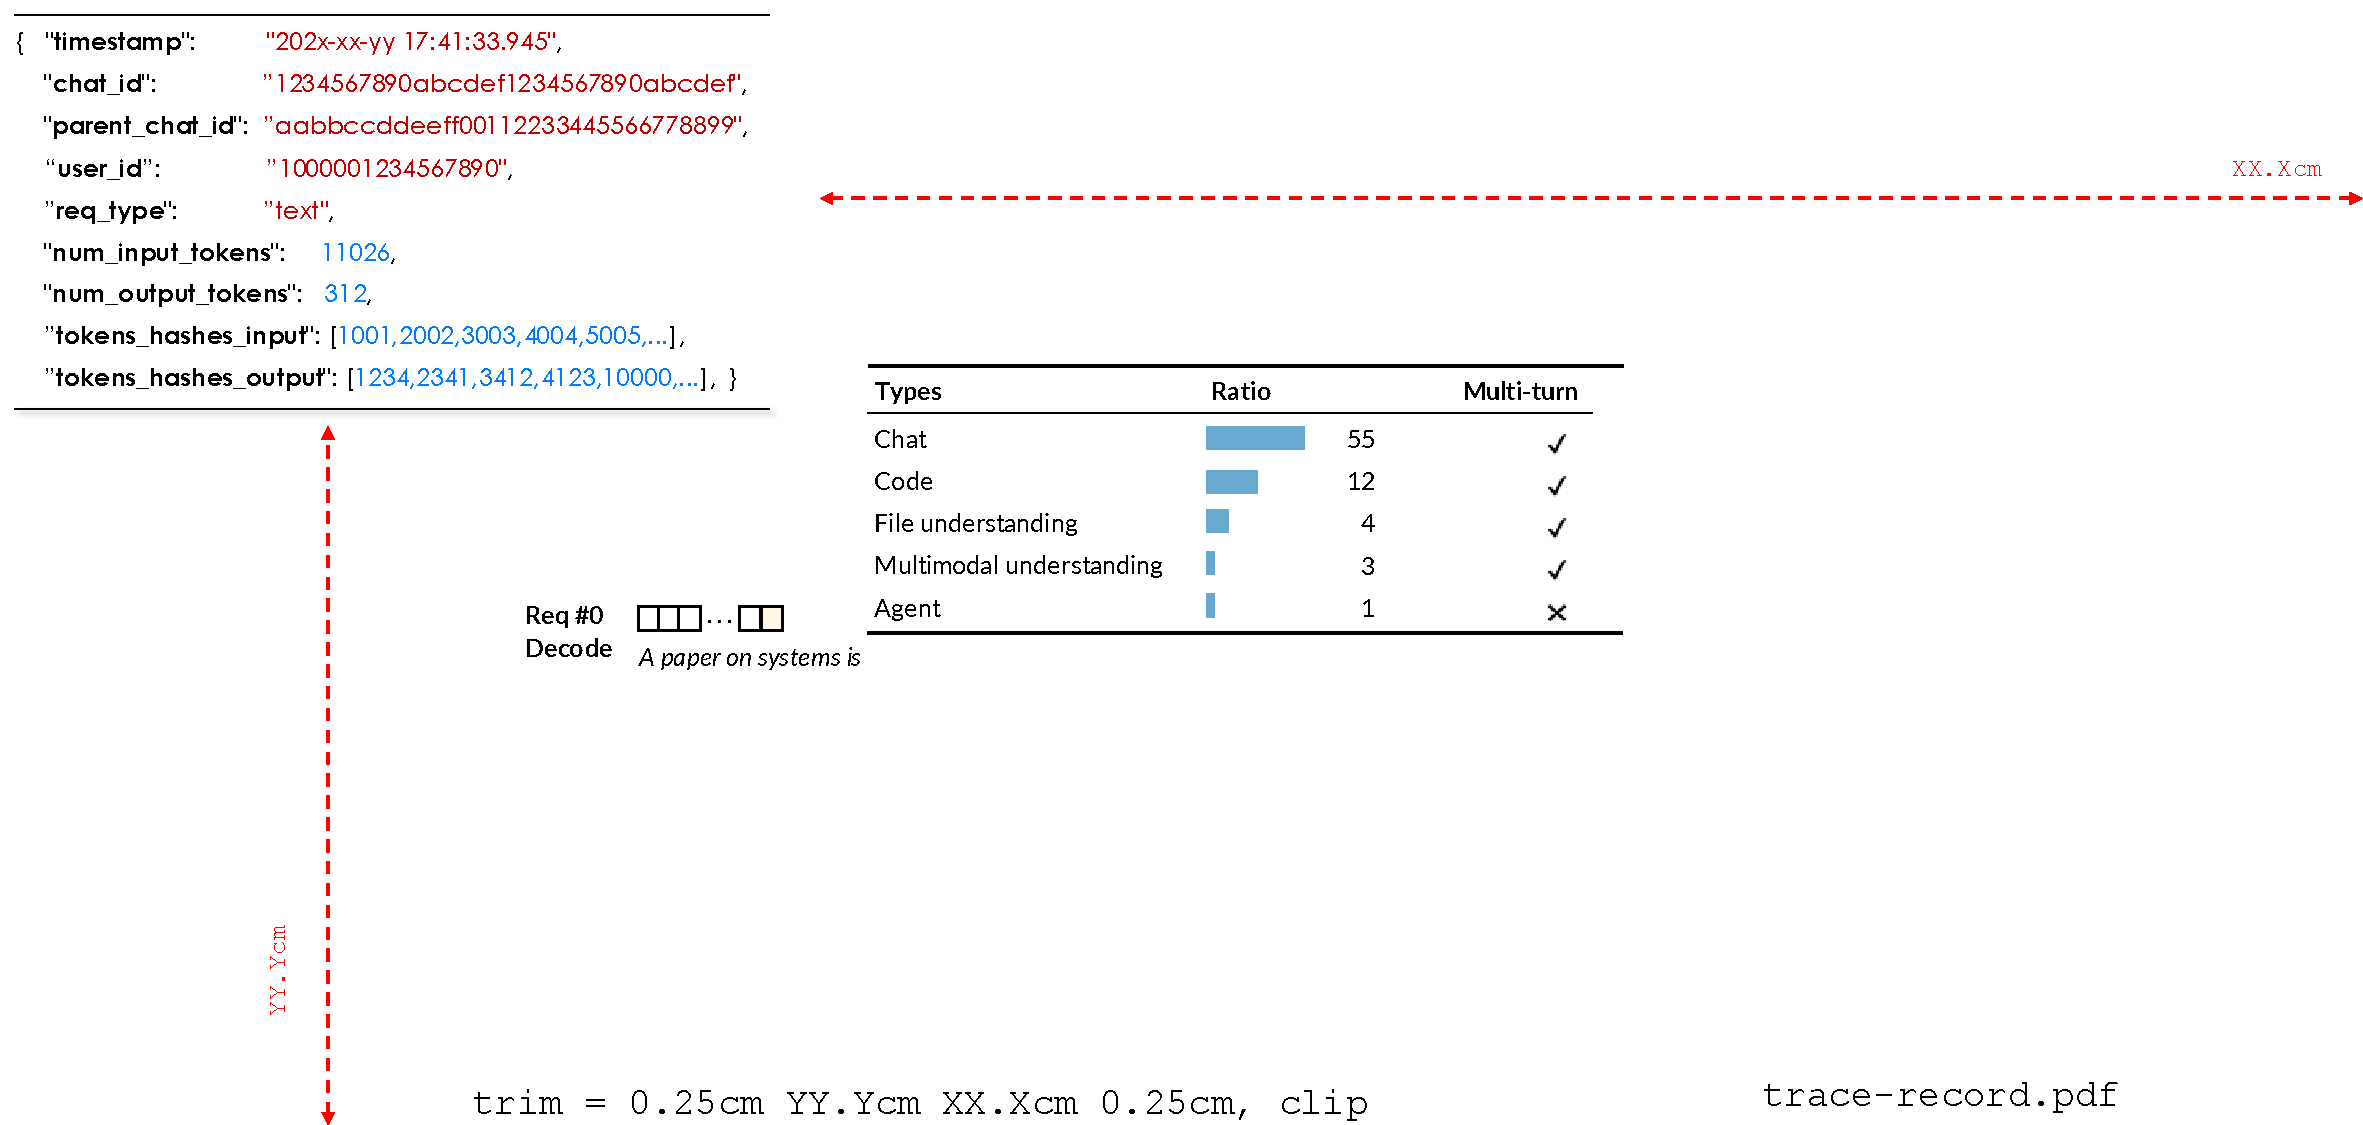
\includegraphics[width=\columnwidth,trim=0.25cm 11.9cm 26.6cm 0.25cm,clip]{figs/trace-record.pdf}
    \caption{所收集轨迹记录的一个示例。}
    \label{fig:trace-record}
\end{figure}

我们从\companyfull 的一个服务集群收集并分析了两周（2025 年 2 月和 2024 年 12 月）的 LLM 服务请求轨迹。为简洁起见，每条轨迹各展示一个代表日的结果；在每周的工作日中，结果始终保持一致（见第~\ref{analysis:reuse-evolution} 节）。\textbf{需要注意：}受\company 严格隐私政策限制，我们无法收集每个请求的原始输入和输出。对于某一条轨迹，其中收集的所有请求都由同一个模型服务。

下面先说明服务集群运维团队提供的匿名轨迹记录细节，再突出两条轨迹的差异；二者均代表当前典型的服务工作负载。\fig{fig:trace-record}展示了一条所收集请求的记录布局：

\stitle{1. 时间戳：}服务集群接收请求的时间。

\stitle{2. 对话 ID：}请求的唯一 ID。

\stitle{3. 父对话 ID（多轮服务中）：}对于多轮会话中的请求，服务系统会为每个请求分配父 ID，将其与会话中的前一个请求关联。沿父 ID 回溯，即可识别属于同一会话的所有请求。若父 ID 为空，则该请求是会话的第一轮，本文称之为\emph{单轮请求}；否则，将父 ID 非空的请求称为\emph{多轮请求}。

\stitle{4. 用户 ID：}提交请求的用户唯一 ID。为实现匿名化，这些 ID 被映射到随机选择的域。

\stitle{5. 请求类型：}服务网关将 LLM 请求分成五类：\emph{Text}，通过 ChatBot 等界面输入纯文本；\emph{File}，文件分析（例如用 LLM 总结文档内容）；\emph{Multimodal}，通过 OCR 增强处理进行图像理解；\emph{Search}，前端集成网页搜索以增强知识；\emph{API}，通过 OpenAI 兼容接口进行程序化访问~\cite{openaiapi}。

\stitle{6. 输入/输出 token 数：}提供给 LLM 的输入 token 数量，以及模型生成的输出 token 数量。

\stitle{7. 输入/输出 token 的哈希值：}受严格隐私政策约束，运行时系统通过带盐哈希和域重映射生成轨迹。具体而言，收集器使用 SipHash~\cite{SipHash}，以每条轨迹随机生成的盐为每连续四个 token 生成唯一哈希值，再把哈希 ID 重映射为连续自然数。与单 token 哈希相比，这种细粒度哈希既支持更细致的缓存分析，也增强了隐私保护。

\stitle{轨迹 A 与轨迹 B。}
我们收集了代表两类典型 LLM 服务工作负载的轨迹 A 和 B。轨迹 A 表示常见的 to-C（消费者）场景，用户通过云平台构建的服务与模型交互，即 ChatBot（Text）或 File、Multimodal、Search 服务。to-C 工作负载的一个关键特征是通常有人参与闭环。轨迹 B 表示 to-B（企业）工作负载，企业用户在计算机程序中调用云平台托管的 OpenAI 兼容 API 与 LLM 交互~\cite{openaiapi}。API 调用对企业用户十分重要，因为它使用户能够系统地利用 LLM 自动完成文档翻译、用户请求分类等任务。轨迹 B 不包含请求类型信息，因为与当前其他厂商提供的 LLM 接口~\cite{openaiapi,genimiapi,claudeapi}类似，这些信息在客户端被拼接到请求中。

\subsection{真实世界中的 {\kvcache} 复用分析}
\label{sec:workload-patterns}

\begin{figure}[!t]
    \centering
    \includegraphics[width=\linewidth]{./data/motiv-cache-hit\figsuffix}
    \caption{一天内真实 LLM 服务工作负载中，{\kvcache} 缓存的理想命中率分析。访问块数与命中块数均经过归一化。}
    \label{fig:motiv-cache-hit}
\end{figure}

\nospacestitle{有多少 {\kvcache} 可以复用？}
\fig{fig:motiv-cache-hit}展示了两条轨迹在缓存容量无限假设下的理想命中率。LLM 工作负载确实可以从缓存中受益：轨迹 A 与 B 的命中率分别为 62\,\% 和 54\,\%。命中率按如下方式计算：若一条轨迹中 LLM 原本需要计算的 {\kvcache} 块总数为 $N$，命中率为 62\,\% 意味着其中 62\,\% 的块可以复用先前请求计算并缓存的 {\kvcache}。尽管理想命中率很高，它仍低于合成工作负载中报告的命中率（例如超过 80\,\%~\cite{DBLP:journals/corr/abs-2403-14401,sglang,cachedattention}）。

\begin{figure}[!t]
    \centering
    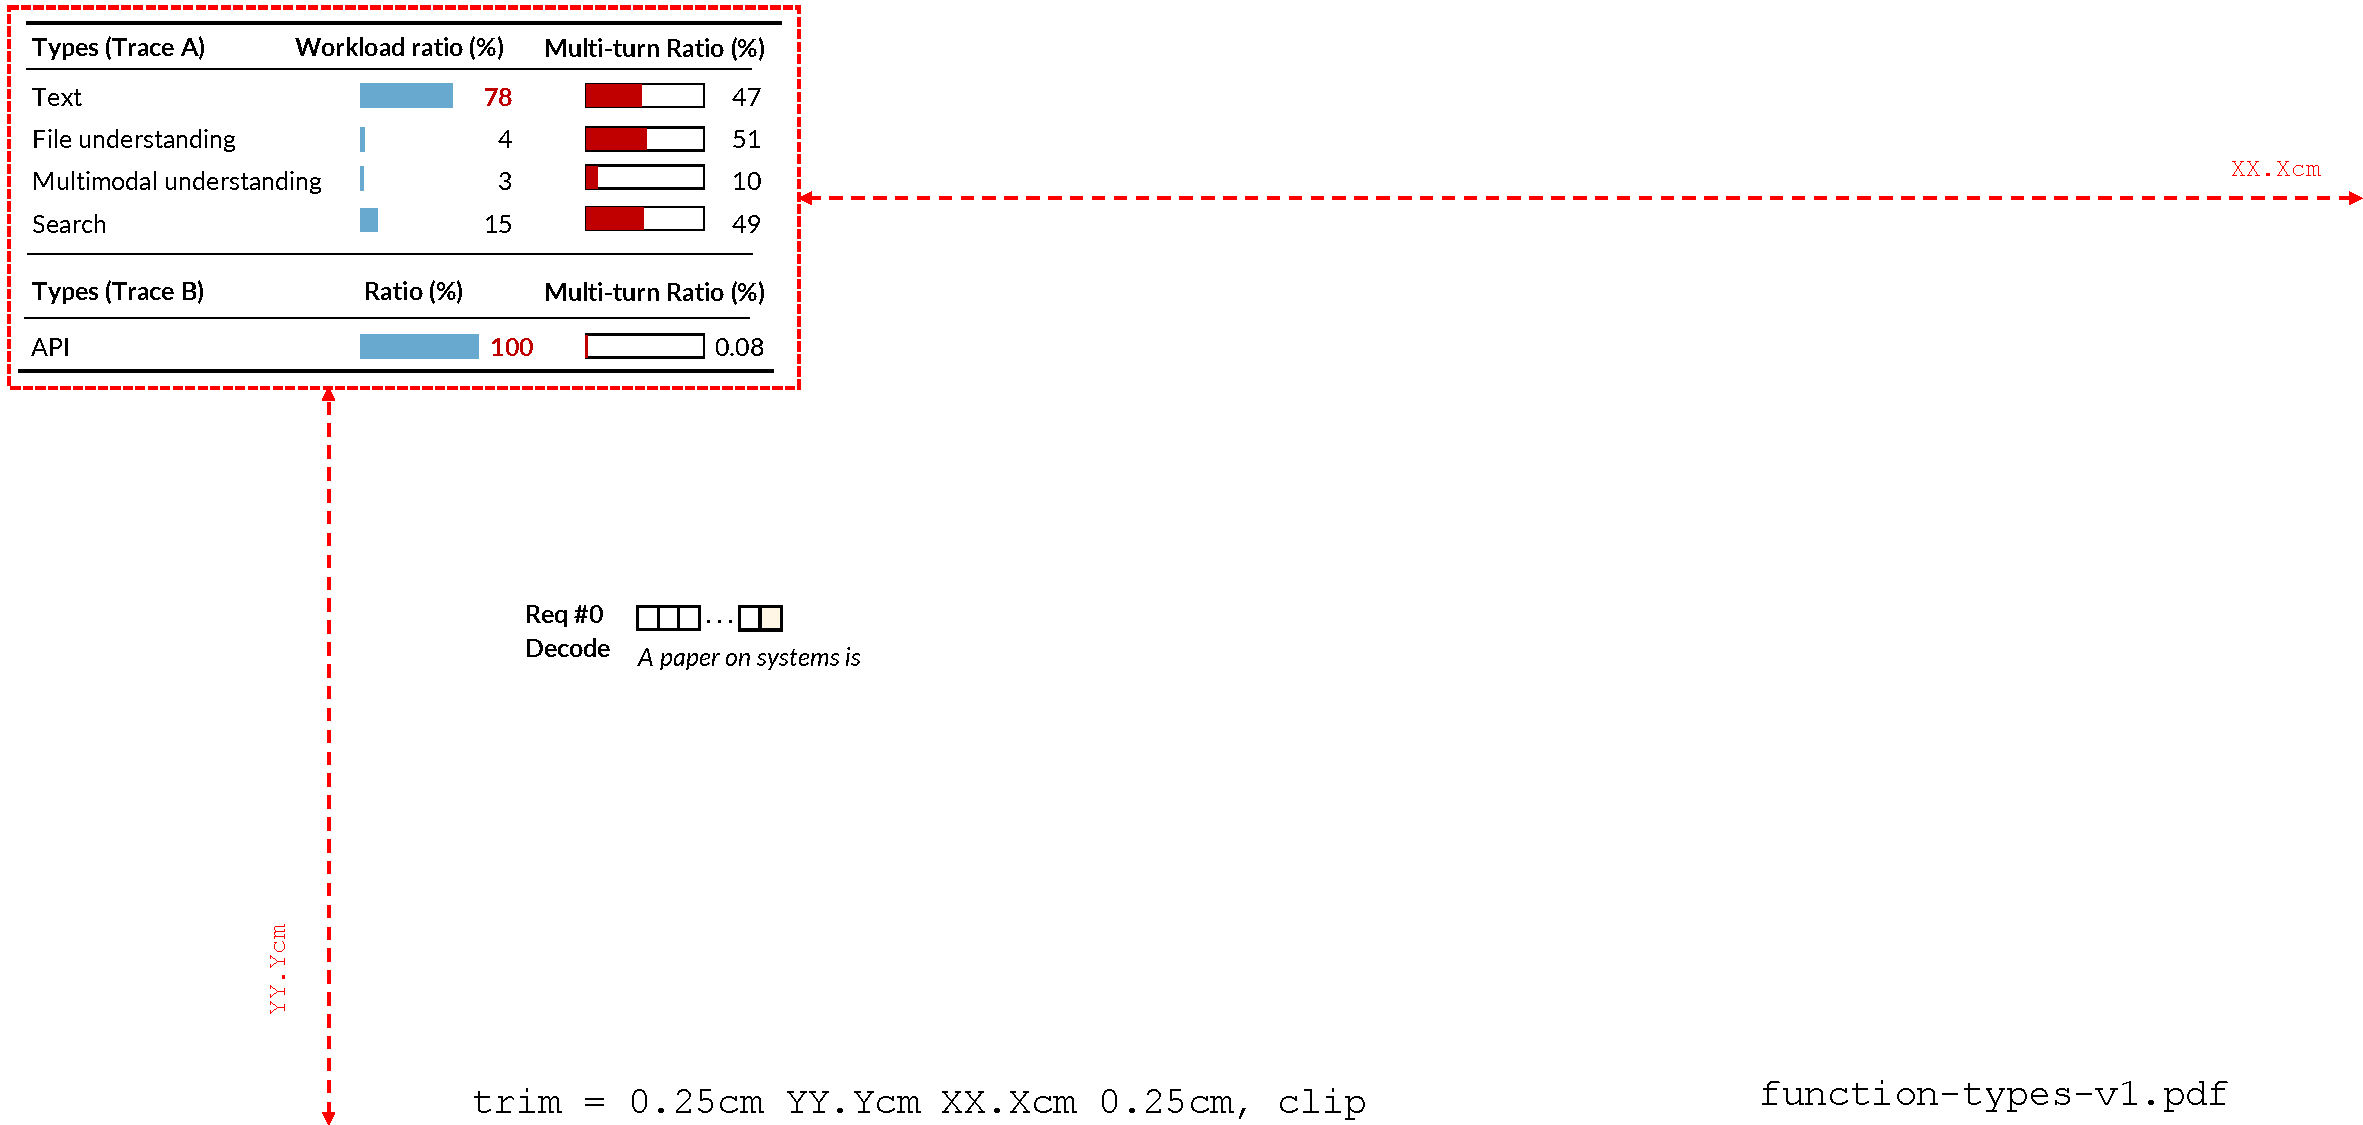
\includegraphics[width=.96\columnwidth,trim=0.25cm 12.54cm 26.9cm 0.25cm,clip]{figs/function-types-v2.pdf}
    \caption{所收集轨迹中的工作负载类型与请求多轮比例。}
    \label{fig:motiv-workload-type}
\end{figure}

\stitle{单轮请求与多轮请求对 {\kvcache} 复用同等重要。}
人们通常认为，多轮请求是缓存命中的主要贡献者~\cite{DBLP:journals/corr/abs-2403-14401,cachedattention}，但对 to-B 工作负载（轨迹 B）并非如此。\fig{fig:motiv-workload-type}展示了各请求类型的占比及其多轮比例。轨迹 A 以聊天机器人发送的请求为主（78\,\%），而除 Multimodal 外，各请求类型的多轮比例相近（47--51\,\%）。轨迹 B 仅包含 API 请求，多轮比例可以忽略不计（低于 0.1\,\%）；即便如此，其中单轮请求仍贡献了总缓存命中的 97\,\%。

单轮 API 请求在 to-B 工作负载中主导命中有两个原因。第一，LLM API 请求通过公共系统提示词共享 {\kvcache}。具体而言，每个请求由两部分构成：（1）给出任务指令的系统提示词（例如文档翻译规范）；（2）包含请求特定数据的用户提示词（例如目标文档）。程序发起 API 调用时~\cite{DBLP:conf/osdi/LinHZ00CQ24}，通常会在程序中硬编码相同的系统提示词，因此即使请求均为单轮，也能跨请求共享 {\kvcache}。第二，API 请求的提交速率往往很高（例如 $>10$ QPS），使同一系统提示词对应的共享 {\kvcache} 得以频繁复用。

\begin{figure}[!t]
    \centering
    \includegraphics[width=\linewidth]{./data/cross-hit\figsuffix}
    \caption{一个用户能否命中另一个用户缓存的 {\kvcache}。颜色越深，归一化命中次数越高。由于轨迹提供方服务的用户很多，为避免对角线过细，图中对其进行了放大。}
    \label{fig:motiv-cross-hit}
\end{figure}

\stitle{跨用户 {\kvcache} 命中十分罕见。}
\fig{fig:motiv-cross-hit}在无限容量 {\kvcache} 缓存假设下，展示了用户之间缓存命中的热力图；颜色越深表示归一化命中次数越多。可以看到，对每个用户而言，大多数命中来自自己提交的请求（即对角线）。用户自然会复用自身请求中的 {\kvcache}，既可能通过多轮对话，也可能通过程序针对同一任务、使用相同系统提示词调用 API；而极低的用户间命中率表明，用户更倾向于自定义系统提示词，而不是采用第三方提示词库~\cite{prompt-library}提供的模板。因此，在设计 {\kvcache} 系统时，本文建议更关注用户内 {\kvcache} 复用，而非用户间复用~\cite{promptcache,sglang,DBLP:journals/corr/abs-2404-12457,DBLP:conf/sigcomm/LiuLCRHZDY0AMHH24}。

\begin{figure}[!t]
    \centering
    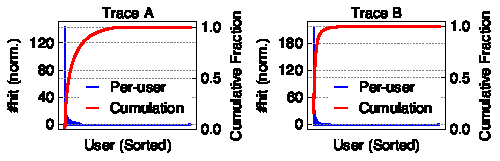
\includegraphics[width=\linewidth]{./data/user-hit-distribution.pdf}
    \caption{无限缓存的理想设置下，不同用户贡献的归一化命中次数。}
    \label{fig:motiv-user-hit}
\end{figure}

\begin{figure}[!t]
    \centering
    \includegraphics[width=\linewidth]{./data/user-distribution\figsuffix}
    \caption{不同用户的归一化请求数。}
    \label{fig:motiv-user-count}
\end{figure}

\stitle{{\kvcache} 复用呈偏斜分布。}
\fig{fig:motiv-user-hit}展示了不同用户贡献的 {\kvcache} 缓存命中及其累计值。命中模式高度偏斜：轨迹 A 中 19\,\% 的用户请求、轨迹 B 中 4\,\% 的用户请求，贡献了超过 90\,\% 的 {\kvcache} 块命中。偏斜来自两个因素。第一，请求在用户之间分布不均，轨迹 B 尤为明显。\fig{fig:motiv-user-count}展示了不同用户发送请求数的归一化值：轨迹 B 中 15\,\% 的用户（头部用户）贡献了 90\,\% 的请求。由于 {\kvcache} 命中主要发生在同一用户发出的请求之间（见\fig{fig:motiv-cross-hit}），请求数的偏斜自然会导致类似的命中偏斜。第二，即使不同用户发送的请求相对均匀，各用户的 {\kvcache} 命中数仍有显著差异。如\fig{fig:motiv-user-count}所示，轨迹 A 的请求分布偏斜程度适中：19\,\% 的用户产生 50\,\% 的请求，72\,\% 的用户产生 90\,\% 的请求；尽管如此，{\kvcache} 命中依然偏斜。作者推测，这源自用户参与多轮请求的倾向不同。

\subsection{多轮请求特征分析}
\label{sec:multi-turn-features}

首先考察多轮请求的特征，因为它们仍然主导 to-C 工作负载中的 {\kvcache} 复用。轨迹 B 中多轮请求十分罕见，因此不报告其对应结果。

\begin{figure}[!t]
    \centering
    \includegraphics[width=\linewidth]{./data/multi-turn-A\figsuffix}
    \caption{轨迹 A 中多轮请求的轮次数分布。}
    \label{fig:motiv-multi-turn-numbersx}
\end{figure}

\stitle{多轮请求具有高度可变性。}
我们观察到两类可变性。第一，不同会话的轮数差异显著。\fig{fig:motiv-multi-turn-numbersx}展示了轨迹 A 中的轮数分布：54\,\% 的请求是单轮请求，第 50 与第 90 百分位轮数分别为 1 和 5。该分布具有长尾，最长会话包含 232 轮，是中位数的两个数量级（232 倍）。

\begin{figure}[!t]
    \centering
    \includegraphics[width=\linewidth]{./data/user-turn-number\figsuffix}
    \caption{每个用户所发送请求的平均轮数（上）与标准差（下）。用户分别按平均轮数（上）和标准差（下）排序。}
    \label{fig:motiv-user-turn-number}
\end{figure}

第二，多轮请求分布在用户层面存在显著差异。\fig{fig:motiv-user-turn-number}表明，除少量头部用户外，大多数用户的平均轮数相近；轮数最高的 10\,\% 用户比总体平均值高 8.9 倍。此外，轮数的标准差差异很大，范围从 1 到 44。这表明用户交互模式多样：有些用户的轮数变化很大，另一些则保持稳定。

\begin{figure}[!t]
    \centering
    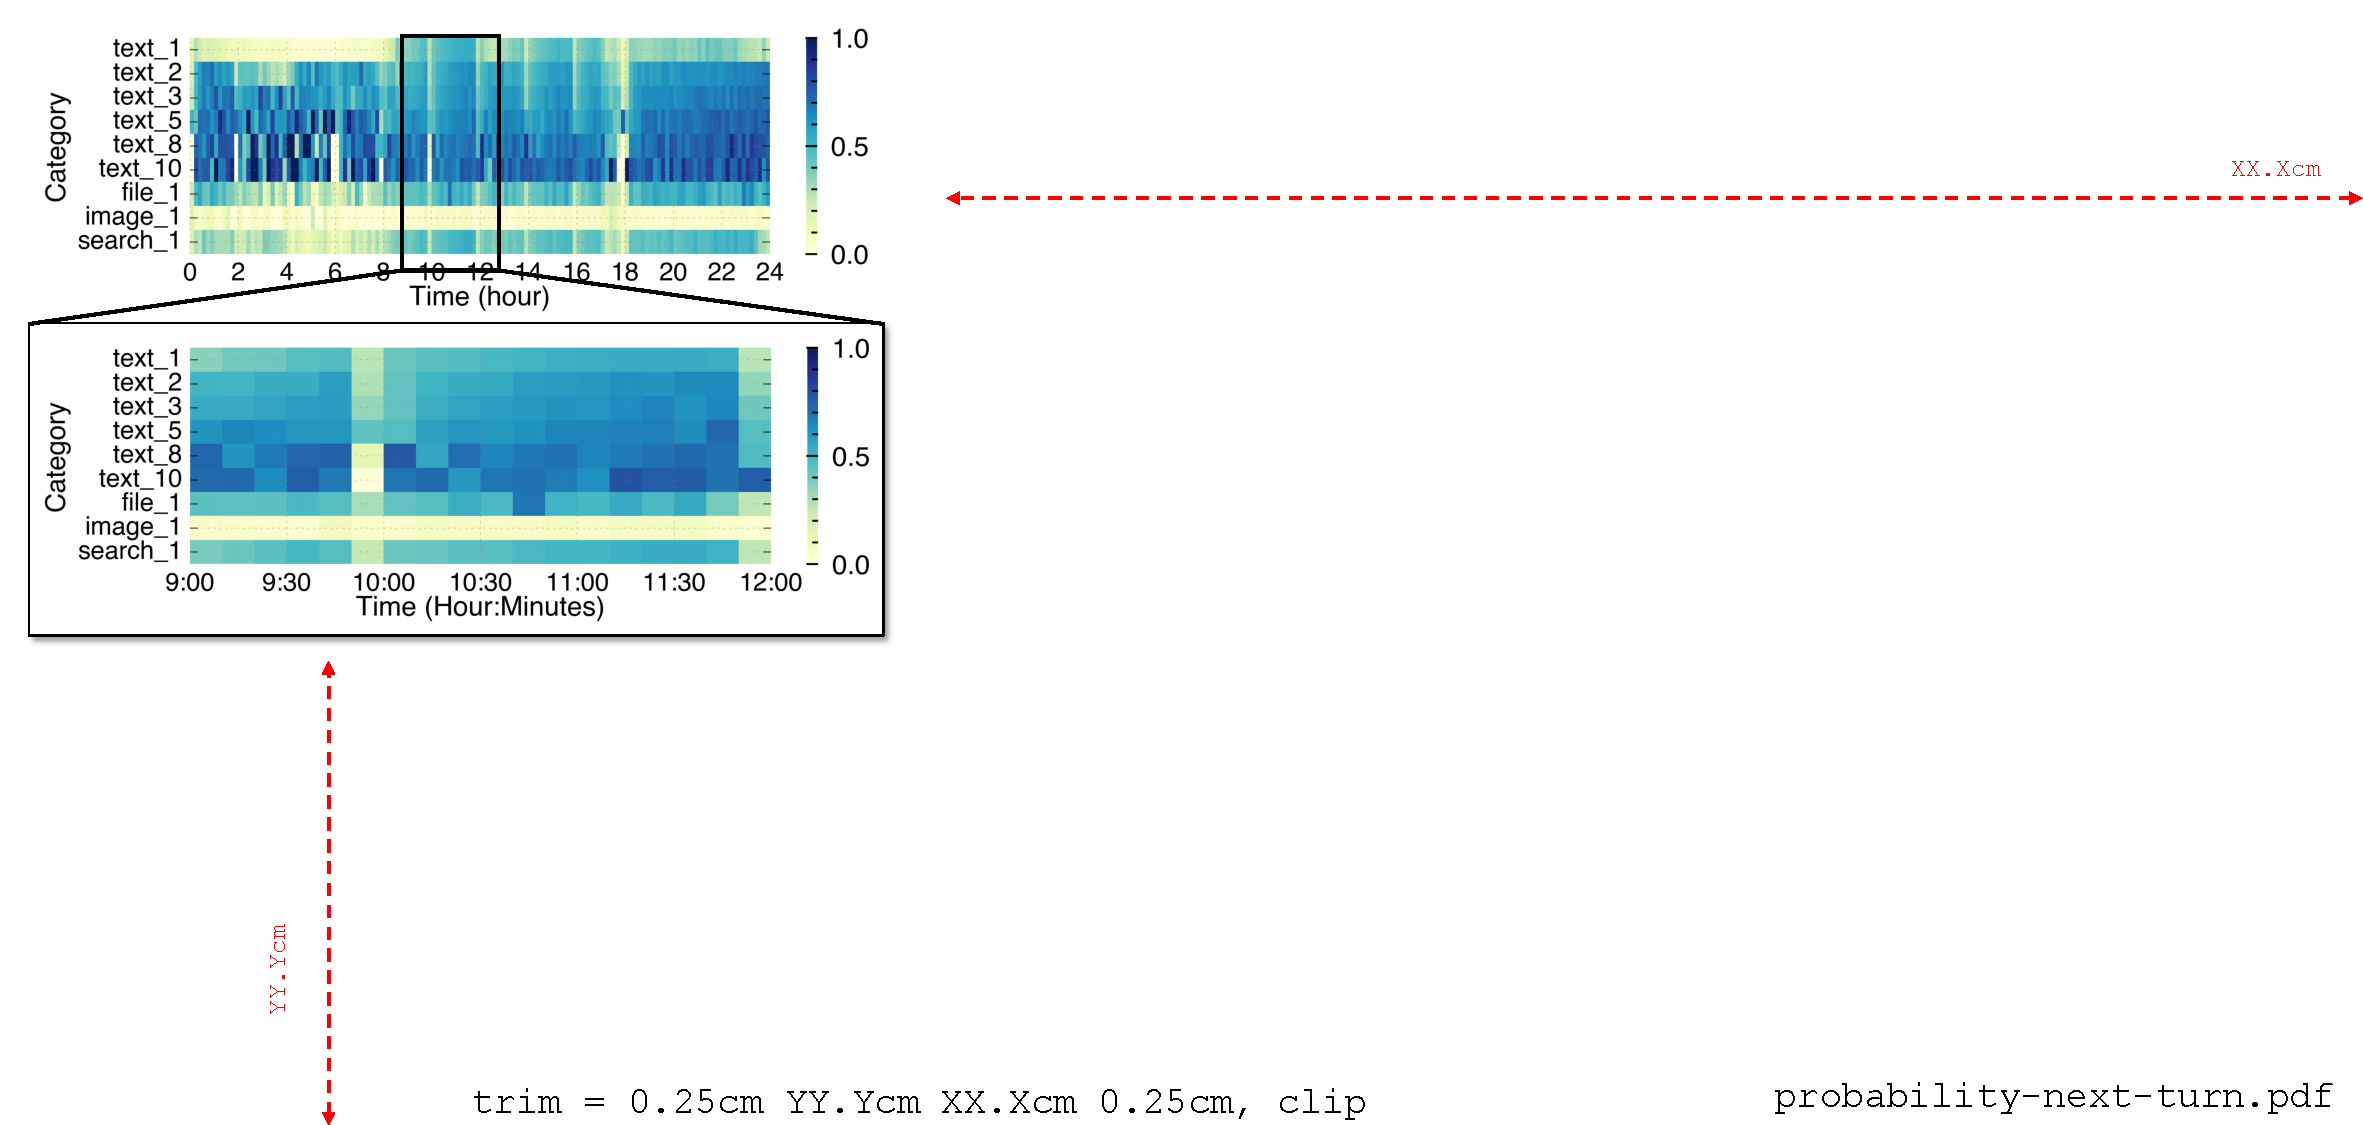
\includegraphics[width=.96\columnwidth,trim=0.25cm 7.9cm 24.1cm 0.25cm,clip]{figs/probability-next-turn.pdf}
    \caption{不同请求类型发起下一轮请求的频率如何随时间变化。横轴为时间线，工作负载类别按流行度排序。}
    \label{fig:motiv-next-turn-probability}
\end{figure}

\stitle{给定工作负载类别和时间区间后，发起下一轮请求的概率可预测，而且不同请求类别的概率不同。}
请求类别同时包含原始请求类型（例如 Text、Search）和请求轮次，即 1 轮 Text（单轮文本请求）与 2 轮 Text 被视为不同类别。\fig{fig:motiv-next-turn-probability}以热力图展示了发起下一轮请求的概率在长时间区间（24 小时）内的变化，以及短时间区间（3 小时）的局部放大；颜色强度表示一个时间窗口（10 分钟）内分析得到的频率。可以看到，虽然不同请求类别的频率不同（表现为竖向色带），但在某一具体类别内，发起下一轮请求的频率在一小时区间内保持稳定（表现为横向色带）。作者将其归因于：给定特定时间区间与请求类别时，{\kvcache} 复用的概率分布相当固定；第~\ref{sec:motiv-temporal-spatial} 节对此作进一步说明。有趣的是，不同请求类别发起下一轮请求的频率确有差异。例如，与多轮请求（均值为 0.8）相比，单轮请求发起下一轮的频率显著更低（均值为 0.5）。

\subsection{时间与空间局部性分析}
\label{sec:motiv-temporal-spatial}

\begin{figure}[!t]
    \centering
    \includegraphics[width=\linewidth]{./data/temporal\figsuffix}
    \caption{轨迹 A 和 B 中所有请求的 {\kvcache} 复用时间分布。}
    \label{fig:motiv-temporal}
\end{figure}

时间局部性可以通过分析复用时间分布来刻画；复用时间是一个 {\kvcache} 块被另一请求复用时的时间间隔。

\stitle{{\kvcache} 复用时间很短。}
\fig{fig:motiv-temporal}展示了两条轨迹的 {\kvcache} 复用时间分布。两种工作负载的复用时间通常都很短：轨迹 A 中 80\,\% 的复用时间小于 10 分钟，轨迹 B 中则小于 10 秒。二者差异来自生成请求的交互方式不同，分别为人在闭环与计算机在闭环。

\begin{figure}[!t]
    \centering
    \includegraphics[width=\linewidth]{./data/temporal-workload\figsuffix}
    \caption{轨迹 A 和 B 中单轮请求的 {\kvcache} 复用时间分布；轨迹 B 只有一种请求类别（API）。}
    \label{fig:motiv-temporal-workload}
\end{figure}

\begin{figure}[!t]
    \centering
    \includegraphics[width=\linewidth]{./data/time-between-turn\figsuffix}
    \caption{轨迹 A 和 B 中多轮请求的 {\kvcache} 复用时间分布；轨迹 B 只有一种请求类别（API）。}
    \label{fig:motiv-time-between-turns}
\end{figure}

\stitle{不同工作负载类型具有不同的时间局部性。}
第一，在 to-C 工作负载中，单轮请求的局部性低得多；to-B 工作负载则相反。\fig{fig:motiv-temporal-workload}中间的子图报告了两条轨迹中一个单轮请求能否被另一单轮请求复用。可以看到，轨迹 A 中可复用的单轮请求少于 30\,\%，而轨迹 B 中超过 50\,\% 的请求可以复用。

第二，不同请求类型呈现不同的时间局部性。\fig{fig:motiv-time-between-turns}按请求类型展示多轮请求的复用时间分布。聊天请求（Text）的复用时间长于图像理解（Multimodal），但短于文件理解（File）。这源自工作负载自身特征：与处理日常对话输出相比，用户通常需要更多时间处理基于文件内容生成的复杂 LLM 输出；反之，视觉信息处理比文本处理更快~\cite{rock2010your}，因此图像任务的复用时间更短。最后，Search 工作负载的复用时间第二长，因为用户常常需要大量时间分析搜索结果。

\begin{figure*}[!t]
    \centering
    \includegraphics[width=\linewidth]{./data/reuse-time-probability-distribution-hist-new\figsuffix}
    \caption{{\kvcache} 块复用时间概率分布的经验分析。各列对应不同请求类别；第一行是在高流量（白天）下的分布，第二行是在低流量（夜间）下的分布，第三行比较不同日期但具有相似流量模式时的分布。}
    \label{fig:motiv-reuse-time-probability-hist}
\end{figure*}

\stitle{给定时间段和请求类别后，{\kvcache} 复用时间的概率分布服从指数分布。}
\label{analysis:block-reuse-probability}
\fig{fig:motiv-reuse-time-probability-hist}给出了不同请求类别中 {\kvcache} 块的复用时间概率分布。对每个类别，我们测量其 {\kvcache} 在缓存后的特定时间间隔被复用的可能性；这些分布通过统计请求执行后每一秒发生的复用事件频率绘制。

结果带来三项关键观察。第一，给定请求类别后，指数分布能够很好地拟合复用概率。第二，概率具有工作负载感知性，即不同请求类别的分布不同，包括请求类型相同但轮次不同的类别（例如 text-1 与 text-2）；这意味着工作负载感知的设计需要区分不同请求类别。第三，流量模式相近的请求具有相似分布。以 text-1 为例，第一行中上午 9:00--10:00 得到的分布与 10:00--11:00 得到的分布相似，却与夜间 3:00--4:00 得到的分布（第二行）明显不同；不同日期之间的分布也相似（第一行与第三行）。第一和第三项观察共同表明，可以使用最近的历史数据获得某一请求类别的分布。

\begin{figure}[!t]
    \centering
    \includegraphics[width=\linewidth]{./data/spatial-v1\figsuffix}
    \caption{两条轨迹的总体空间局部性。}
    \label{fig:motiv-spatial}
\end{figure}

\begin{figure}[!t]
    \centering
    \includegraphics[width=\linewidth]{./data/spatial-multi-traceC\figsuffix}
    \caption{轨迹 A 中多轮请求的空间局部性。}
    \label{fig:motiv-spatial-multi}
\end{figure}

\stitle{空间局部性。}
\fig{fig:motiv-spatial}展示了两条轨迹中 {\kvcache} 的总体空间局部性。本文用不同缓存步长（即每个请求中被缓存 token 的比例）以及不同缓存起始 token 偏移量下的理想命中率来刻画空间局部性，由此得到二维热力图。例如，偏移量 $(10\,\%,10\,\%)$ 表示对每个请求，只缓存从 10\,\% token 位置开始的 10\,\% token。

第一，从开头开始缓存时，{\kvcache} 的空间局部性更好。这符合预期，因为只有前缀完全相同的请求才能共享 {\kvcache}（第~\ref{sec:bg} 节）。本文强调这一看似显然的事实，是因为一些 {\kvcache} 优化~\cite{DBLP:journals/corr/abs-2410-03065}会缓存请求尾部 token，通过并行计算与加载隐藏 {\kvcache} 加载时间；但这种方法可能降低空间局部性。尤其是\fig{fig:motiv-spatial-multi}表明，对多轮对话而言，复用缓存中的中间部分几乎没有收益。

\begin{figure*}[!t]
    \centering
    \includegraphics[width=.95\linewidth]{./data/spatial-workload-cd\figsuffix}
    \caption{单轮请求的空间局部性。}
    \label{fig:motiv-spatial-workload}
\end{figure*}

第二，与时间局部性一样，空间局部性也具有工作负载感知性。在\fig{fig:motiv-spatial-workload}中，Text 和 Multimodal 等工作负载表现出明显空间局部性，而 File 与 Search 几乎没有空间局部性。由于无法获得用户输入内容，作者推测原因如下：应用会为 Text 和 Multimodal 工作负载加入固定系统提示词，而 File 与 Search 的系统提示词依赖用户输入。

最后，我们发现，在轨迹 A 中增大步长会提高缓存命中率（\fig{fig:motiv-spatial-multi}），但轨迹 B 并非如此（\fig{fig:motiv-spatial-workload}最后一列）。轨迹 A 中多轮请求会贡献缓存命中，因此为一个请求缓存更多 token 会带来更多命中。轨迹 B 中只有系统提示词贡献缓存命中，所以缓存请求中 50\,\% 的 token 已达到 50\,\% 的峰值命中率。这意味着轨迹 B 中多数系统提示词长度低于请求总长度的 50\,\%，但作者并无详细请求内容来支持这一推测。

\subsection{{\kvcache} 缓存容量需求分析}
\label{sec:analyze-capacity}

确定合适的缓存容量对缓存系统至关重要。不同于传统存储系统，缓存的 {\kvcache} 生命周期短暂，因此识别恰当的容量需求可以节省平台成本。本节采用自底向上的方式分析 {\kvcache} 容量：首先刻画请求 {\kvcache} 生命周期的特征，再分析每个请求的存储用量；两者结合即可估计所需的 {\kvcache} 总容量。

\begin{figure}[!t]
    \centering
    \includegraphics[width=\linewidth]{./data/block-timespan-cdf\figsuffix}
    \caption{两条轨迹中 {\kvcache} 块生命周期的分布。}
    \label{fig:motiv-block-timespan}
\end{figure}

\stitle{{\kvcache} 生命周期短暂且可预测。}
\fig{fig:motiv-block-timespan}分析了 {\kvcache} 块的生命周期。如果一个 {\kvcache} 块此后不再被复用，就称其“死亡”。可以看到，大多数 {\kvcache} 块“存活”时间很短：轨迹 A 中 90\,\% 的 {\kvcache} 块在 612 秒后不再被复用，轨迹 B 中这一数值为 0.3 秒。这与前文分析一致，例如许多多轮请求的复用时间很短（\fig{fig:motiv-temporal}），而多数请求只有少数几轮（\fig{fig:motiv-multi-turn-numbersx}）；一旦多轮请求结束，其 {\kvcache} 就不再复用。尽管存在少数离群值，轨迹 B 中块的生命周期仍更短。与轨迹 A 不同，轨迹 B 中缓存的多数 {\kvcache} 块服务于系统提示词，因而在很久以后仍可能被复用。例如，轨迹 B 中最长生命周期为 1,200 分钟，轨迹 A 中为 800 分钟。

\begin{figure}[!t]
    \centering
    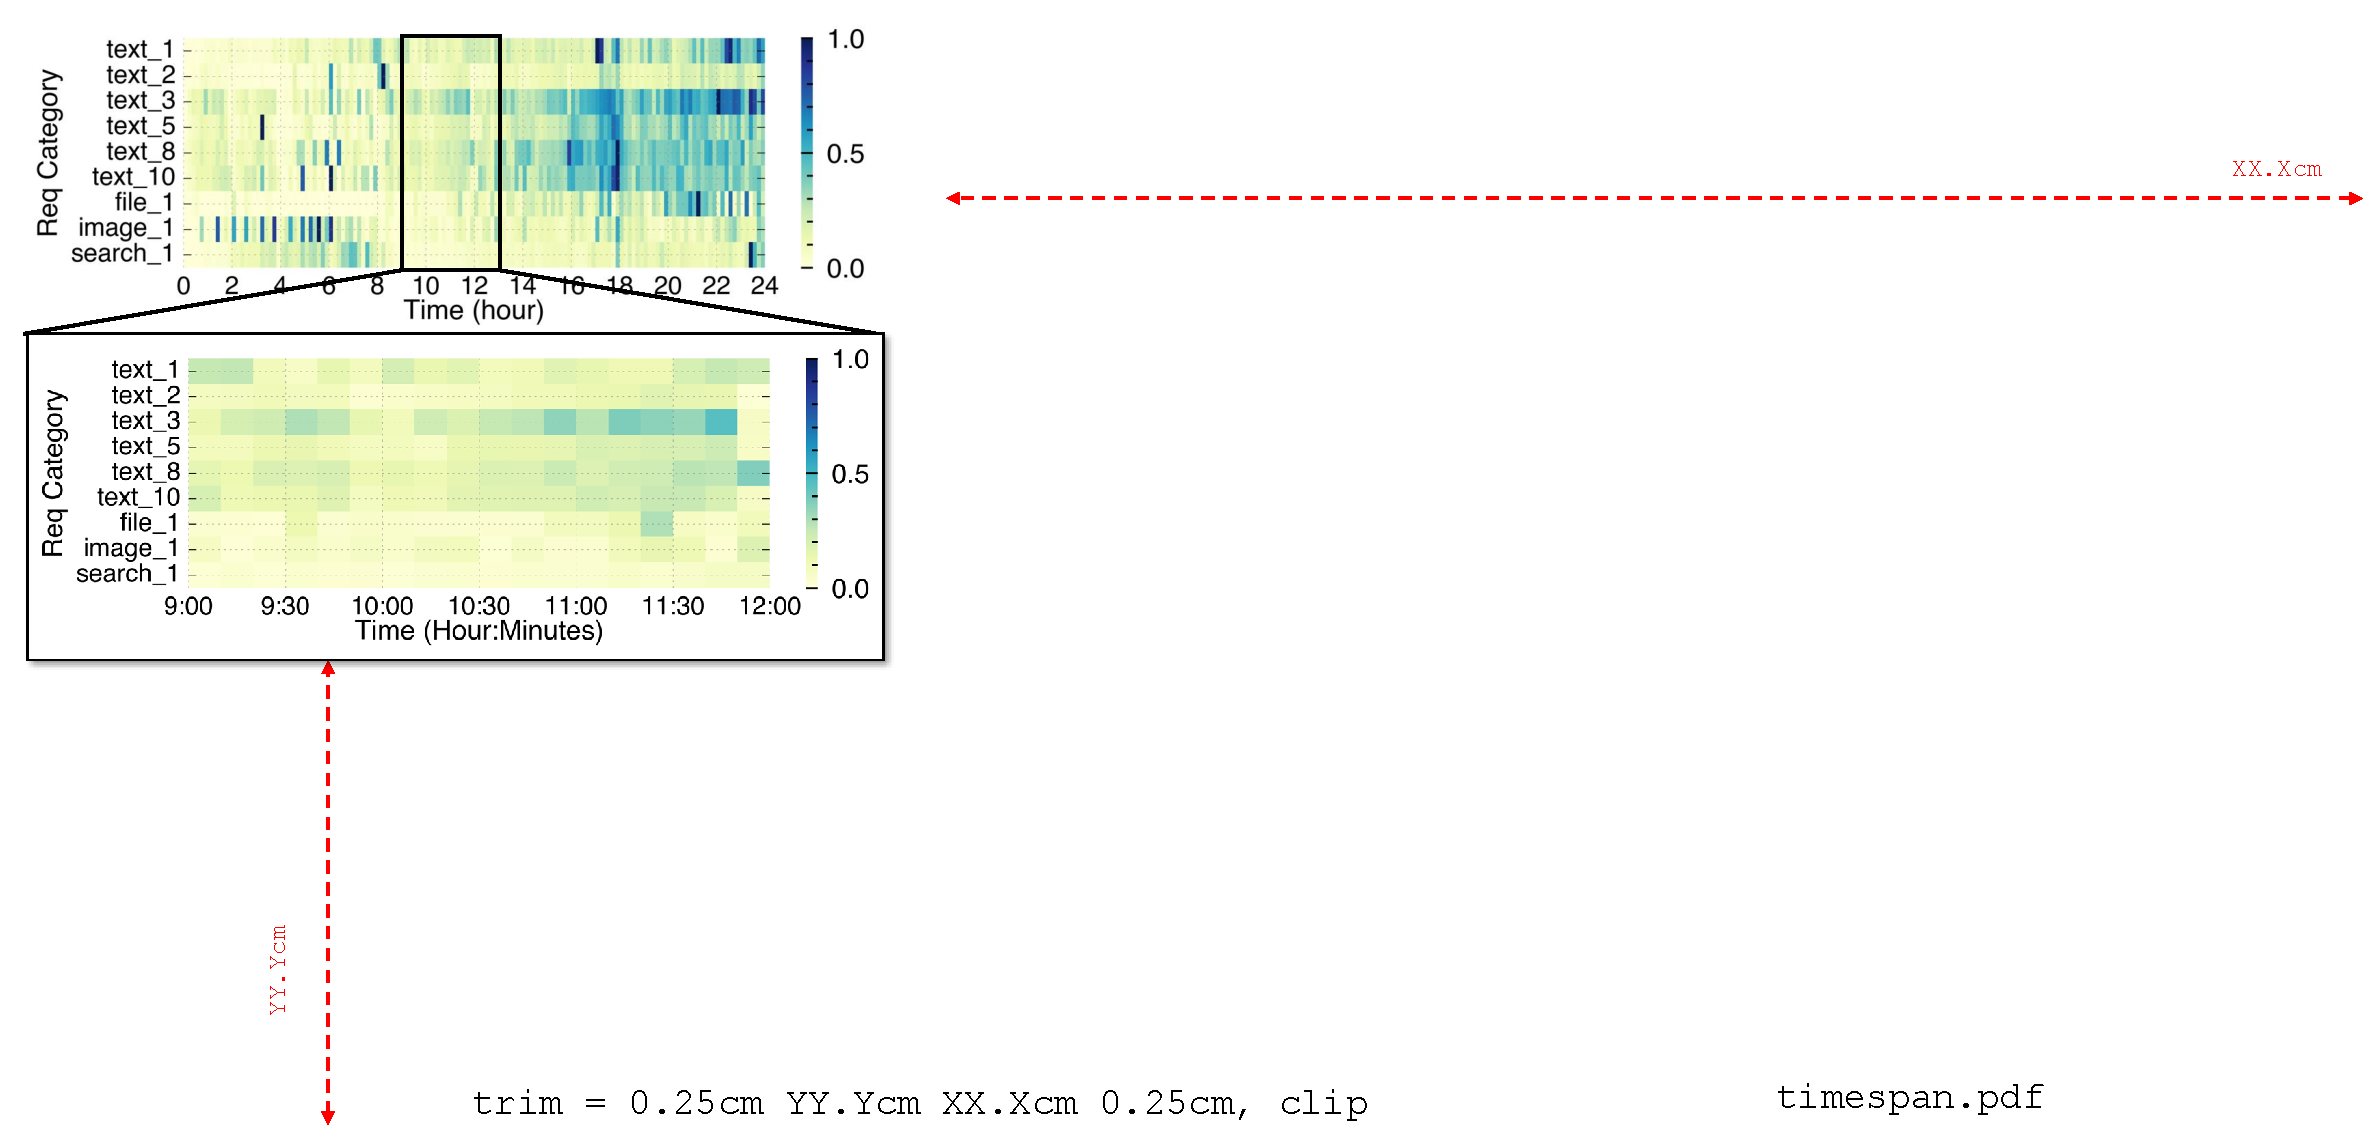
\includegraphics[width=.96\columnwidth,trim=0.25cm 7.85cm 24.1cm 0.25cm,clip]{figs/timespan.pdf}
    \caption{不同请求类别中，{\kvcache} 块的平均生命周期如何随时间变化。横轴为时间线，请求类别按使用量排序。}
    \label{fig:motiv-block-timespan-probability}
\end{figure}

\fig{fig:motiv-block-timespan-probability}进一步展示了不同请求类别中 {\kvcache} 块平均生命周期随时间的变化。图中颜色强度表示归一化生命周期，颜色越深表示 {\kvcache} 块存活越久。尽管平均生命周期在 24 小时时间尺度上随时间变化，但放大到更短时间尺度（上午 9:00--11:00）后，模式相当稳定。这意味着，可以利用历史数据预测 {\kvcache} 块的生命周期，从而缩减 {\kvcache} 缓存并节省成本，因为在高速存储介质（例如 CPU DRAM）中存储 {\kvcache} 的成本很高。

\begin{figure*}[!t]
    \centering
    \includegraphics[width=\linewidth]{./data/size-v2\figsuffix}
    \caption{不同轨迹中\uline{单}轮与\uline{多}轮请求的 {\kvcache} 大小分布。大小相对于可用于服务的 GPU 内存（HBM）进行归一化；各图元组中的数字表示输入和输出长度。}
    \label{fig:motiv-cache-size}
\end{figure*}

\stitle{单请求 {\kvcache} 缓存用量适中。}
考虑缓存时，一个关键因素是待缓存 {\kvcache} 的大小，它与每个请求的输入长度及相应的模型输出长度成正比。\fig{fig:motiv-cache-size}展示了不同轨迹中的请求大小分布。需要注意，本文报告的是相对于一个服务实例中可用于服务该请求的 HBM 所归一化的相对大小\footnote{服务实例是服务一个模型所需的最少 GPU 数。例如，服务 8B 模型只需一块 GPU，而通常服务 72B 模型需要四块 GPU。}，因为相对值能更直观地反映缓存每个请求的 {\kvcache} 所需容量。可用于 {\kvcache} 的 HBM，通过从服务实例中 GPU 的总 HBM 扣除模型参数与激活大小得到。由于单请求 {\kvcache} 大小取决于模型的具体注意力机制，本文报告了采用两种广泛使用注意力方法的三个代表性模型：分组查询注意力（GQA~\cite{DBLP:conf/emnlp/AinslieLJZLS23}）与多头注意力（MHA~\cite{DBLP:conf/nips/VaswaniSPUJGKP17}）。GQA 的 {\kvcache} 内存需求更低。

可以看到，与 HBM 相比，{\kvcache} 的总体大小适中。以轨迹 A 为例，在 Qwen2-7B 等 GQA 模型上，占主导的 Text 请求类型中，单轮请求在第 50、90、99 百分位的 HBM 用量分别为 0.09\,\%、0.15\,\%、0.37\,\%，多轮请求分别为 0.36\,\%、1.31\,\%、2.21\,\%；单轮与多轮请求的平均用量分别为 0.09\,\% 和 0.56\,\%。用量之所以较小，是因为每个 token 只消耗数 MB，而生产轨迹中的请求往往较短：Qwen2-7B 每 16 个 token 消耗 0.875\,MB {\kvcache}，单轮与多轮请求的平均 token 总长度（输入加输出）分别为 973 与 5,953。对于其他模型，Llama3-70B 虽然也采用 GQA，但由于每个实例的 GPU 数量增长较慢，其 HBM 用量略高：参数规模增长 10 倍，而本文测量配置中的 GPU 数仅增长 4 倍。最后，MHA 模型的用量最高，因为每个 token 的 {\kvcache} 更大。值得注意的是，近期开放模型倾向于采用 GQA，或采用 MLA~\cite{liu2024deepseek}等每 token {\kvcache} 更少的注意力机制。

考虑到每个服务实例通常每秒处理数个请求，上述刻画意味着实例能够以适中的时长缓存请求。例如，对 Qwen2-7B，假设一块 GPU 每秒可处理 5 个请求，并按每请求平均占用 0.32\,\% HBM 计算（由 Text 请求 47\,\% 的多轮比例推导），至少需要 1 分钟才会占满 HBM。该时长落在许多场景（例如 API）中 {\kvcache} 的复用距离内。需要注意的是，在实际设置中，由于尾部请求（例如确实存在上下文超过 12,000 token 的长请求），可能达不到如此长的复用时长；同时，为提高计算利用率，LLM 服务系统通常会以大批次服务请求。

\begin{figure}[!t]
    \centering
    \includegraphics[width=\linewidth]{./data/opt-cache-space\figsuffix}
    \caption{不同模型与轨迹中，达到理想缓存命中率所需的 {\kvcache} 缓存大小；数据采集于上午 10:00--11:00。}
    \label{fig:motiv-opt-cache-space}
\end{figure}

\stitle{{\kvcache} 缓存所需的总体内存适中。}
本文通过测量在理想淘汰策略下，多大的缓存能够保证理想命中率，来分析所需的 {\kvcache} 缓存容量；理想策略永不淘汰未来还会复用的 {\kvcache}。测量方法如下：在给定时刻处理一个请求时，如果该请求的 {\kvcache} 未来还会复用，就把其大小加入当前 {\kvcache} 用量；同时减去缓存中所有永远不会再复用的 {\kvcache} 大小。一个棘手之处是，需求大小取决于为工作负载部署的服务实例数：若实例过度配置，估计出的需求会偏小。为得到最大需求，本文使用最少的服务实例，即每个实例都以最大 QPS 服务，从而不存在过度配置。

\fig{fig:motiv-opt-cache-space}给出了相对于服务实例总 HBM 归一化后的结果。GQA 模型只需较小缓存容量即可达到理想命中率：在轨迹 A 中，Llama3-70B 所需容量仅为可用于 {\kvcache} 的 HBM 的 4 倍。现代服务集群通常可以满足这一需求，无需远程内存或 SSD 等更多存储层次~\cite{cachedattention}。例如，在包含 8 块 A100 GPU 和 1\,TB CPU 内存的典型设置中，每块 GPU 平均可使用 128\,GB CPU 内存，约为保留给 {\kvcache} 的 HBM 空间的 4 倍。此外，轨迹 B 的 {\kvcache} 容量甚至小于保留的 HBM，因此仅在 GPU 上缓存可能已经足够。

尽管 GQA 需要的缓存很小，仍应注意 MHA 模型确实需要巨量 {\kvcache} 缓存，这是因为其每 token KV 对非常大（见\fig{fig:motiv-cache-size}）。因此，在缓存容量受限时，优化淘汰策略仍然重要。
